\documentclass[12pt, letterpaper]{article}
\usepackage{color}
\usepackage{natbib}
\usepackage{parskip}
\usepackage{amsmath}
\usepackage{amssymb}
\usepackage{graphicx}
\usepackage{listings}
\usepackage{setspace}
\usepackage{geometry}
\usepackage{enumitem}
\usepackage{dirtytalk}
\usepackage{subcaption}
\usepackage{indentfirst}
\usepackage{anyfontsize}
\usepackage[utf8]{inputenc}

\parindent=0.5in

\graphicspath{{./imgs/}}

\definecolor{codegray}{rgb}{0.2,0.2,0.2}
\definecolor{codepurple}{rgb}{0.58,0,0.82}
\definecolor{backcolor}{rgb}{0.95,0.95,0.92}

\lstdefinestyle{scheme}
  {backgroundcolor=\color{backcolor},
  commentstyle=\color{blue},
  keywordstyle=\color{magenta},
  numberstyle=\tiny\color{codegray},
  stringstyle=\color{codepurple},
  basicstyle=\footnotesize\ttfamily,
  morekeywords={*},
  breakatwhitespace=false,
  breaklines=true,
  captionpos=t,
  keepspaces=true,
  numbers=left,
  numbersep=5pt,
  showspaces=false,
  showstringspaces=false,
  showtabs=false,
  tabsize=2,
  title=\lstname,
  language=Python
}

\lstset{style=scheme}

\doublespace{}
\title{On Splines and Their Use in Computer Graphics and Generating Curves}
\author{Simon Abrelat}
\date{\vspace{-5ex}}

\DeclareUnicodeCharacter{2212}{-}
\begin{document}

\large
{\fontsize{12}{14.4}
  {\singlespace{}
  \pagenumbering{gobble}
  \maketitle
  \begin{center}
  \vspace{4mm}
  002129--0004 \\
  \vspace{4mm}
  Math HL IA \\
  \vspace{4mm}
  May 2019 \\
  \vspace{4mm}
  Words: \\
  \end{center}
  }
}
\newpage

\pagenumbering{arabic}
\begin{abstract}
Splines are used everywhere around us, from fonts to animations. They are the way that computers deal with
curves and because of that have a large range of possible uses. Since they are so useful, there are also a
lot of ways to generate these functions and lots of formats they come in. In general, they are fairly
computationally cheap which makes them so useful and can be extended in a multitude of ways. In this paper,
the goal would be to use splines to smoothly interpolate values either for control or for path generation.
\end{abstract}

\newpage
\tableofcontents
\newpage

\section{Introduction}
Splines are not a specific equation, they are more a class of equations that have similar properties. They are
simply piecewise polynomials, and are often parameterized so that they could \say{loop over themselves} and
break the vertical line test. One of the interesting aspects of splines is that they keep this property even
at low degrees. The word spline is derived from wooden splines that curve given some constraints and are often
used in things like braces for ships. The major benefit of splines is how they are suited for computers.
Almost all curves on a computer from fonts to animation paths are described quickly and accurately by
B\`{e}zier curves and other such splines. This means that these splines are around us all of the time and are
almost invisible if you do not know where to look. There are many different kinds of splines with different
methods of formulation. However, this paper will mostly be focused on Hermite and B\`{e}zier curves.

\section{B\`ezier Curves}
\subsection{Theory}
B\`ezier curves can be made with a linear combination of Bernstein polynomials \citep{ams}. Bernstein
polynomials were first used in the proof of the Stone-Weierstrass theorem which states that every continuous
function defined on a closed interval $[a,b]$ can be approximated as closely as desired by a polynomial
\citep{weierstrass}. A Bernstein polynomial (\ref{eq:BPoly}) is defined by a linear combination of Bernstein
basis functions (\ref{eq:BBasis}).

Bernstein Polynomials:
\begin{singlespace}
  \begin{equation}
    \label{eq:BBasis}
    b_{\nu,n} = {n \choose \nu} x^\nu (1 - x)^{\nu - n}
  \end{equation}
  \begin{equation}
    \label{eq:BPoly}
    B_n(x) = \sum_{\nu = 0}^{n}\beta_\nu b_{\nu,n} (x)
  \end{equation}
  \begin{equation}
    \label{eq:BLimit}
    \lim_{n\to\infty} B_n(f) = f
  \end{equation}
  \begin{small}
		\begin{itemize}[label=]
    	\item $n$: is the degree of the Bernstein function
    	\item $\nu$: is number of the $n+1$ equations of a function of degree $n$ 
		\end{itemize}
  \end{small}
\end{singlespace}

\begin{figure}[ht]
  \caption{Basis functions for different degrees, Listing~\ref{lst:basis}}
  \label{fig:basis}
  \begin{center}
    \begin{subfigure}[b]{.45\linewidth}
      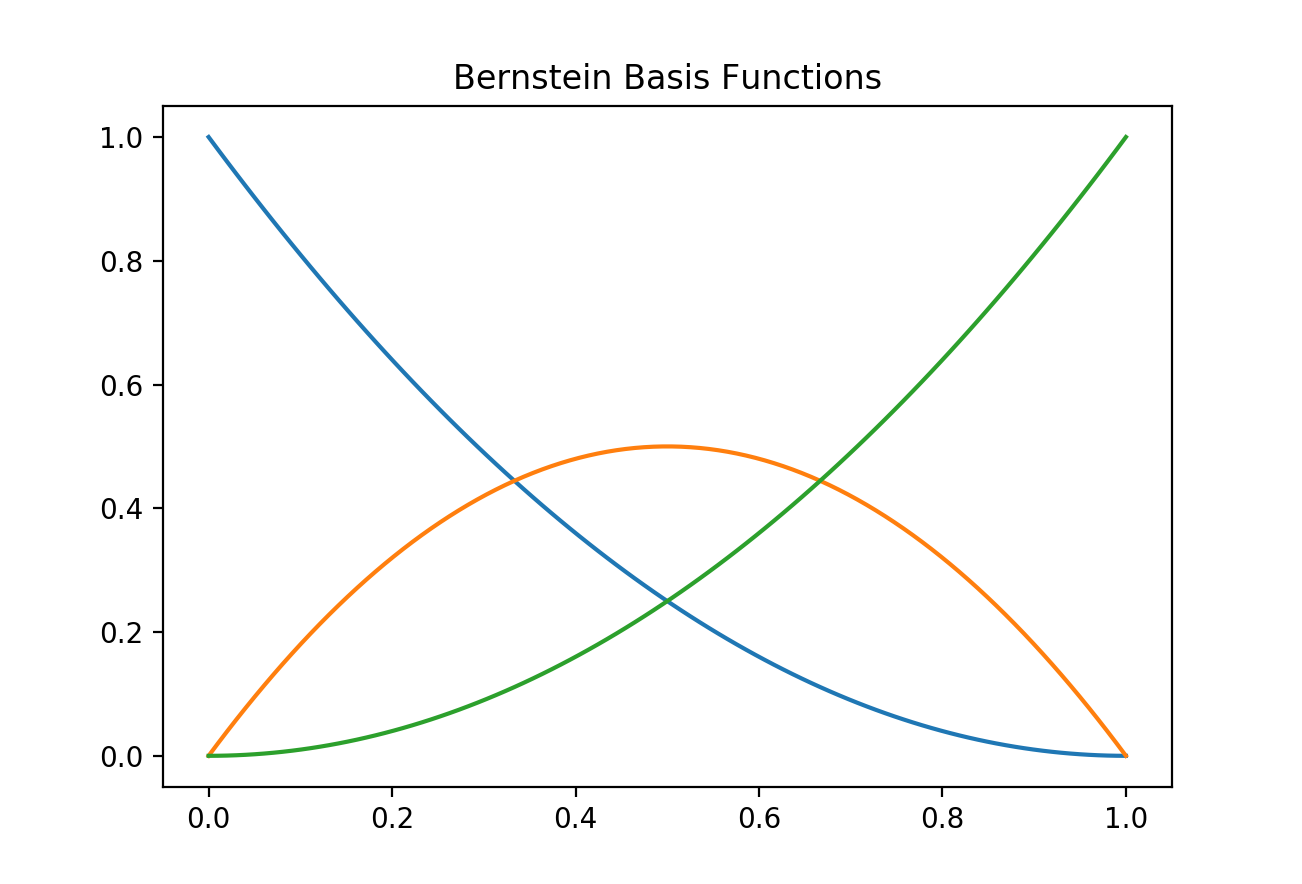
\includegraphics[width=\linewidth]{Basis/basis2}
      \caption{$n=2$}
    \end{subfigure}
    \begin{subfigure}[b]{.45\linewidth}
      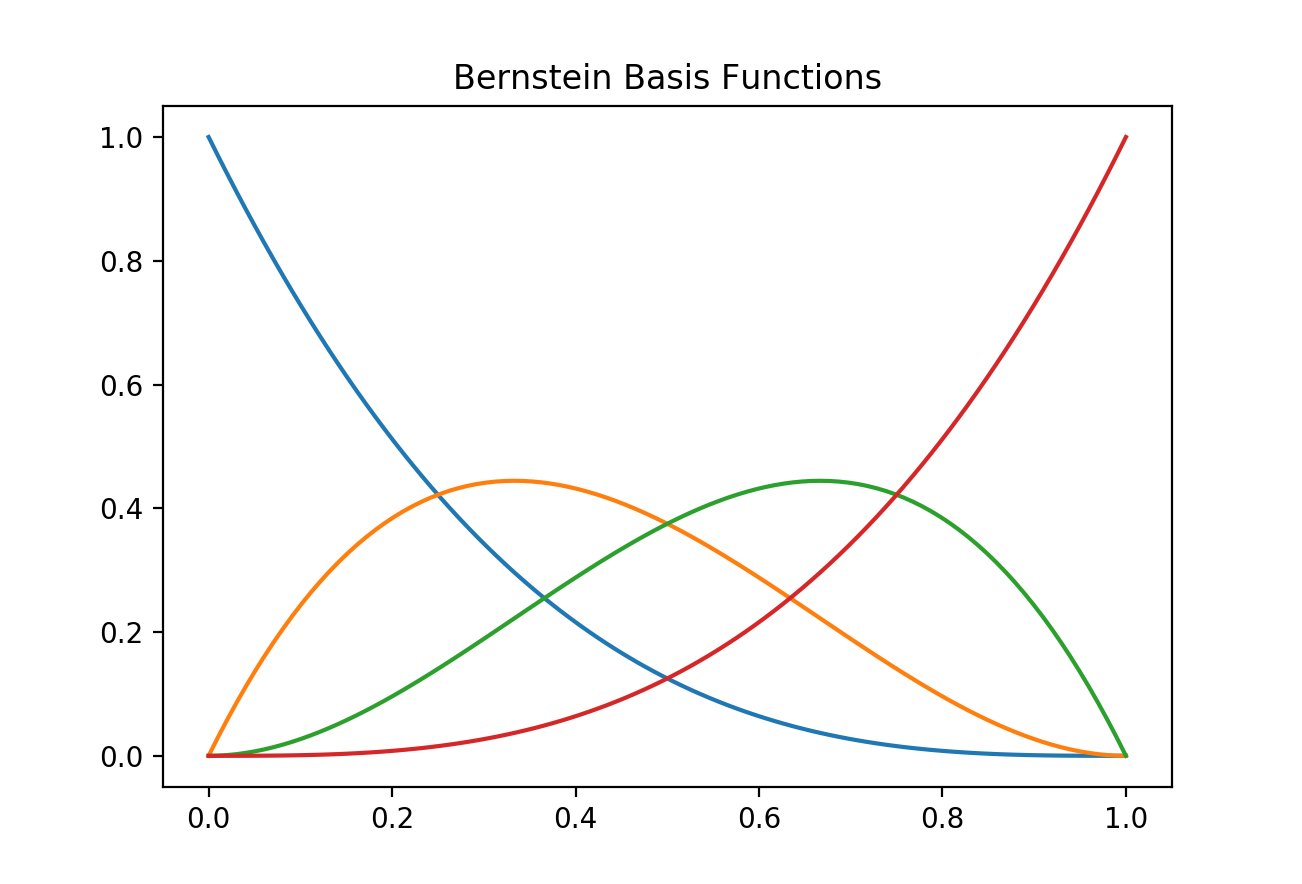
\includegraphics[width=\linewidth]{Basis/basis3}
      \caption{$n=3$}
    \end{subfigure}
  \end{center}
\end{figure}
\begin{figure}[ht]
  \begin{center}
    \begin{subfigure}[b]{.45\linewidth}
      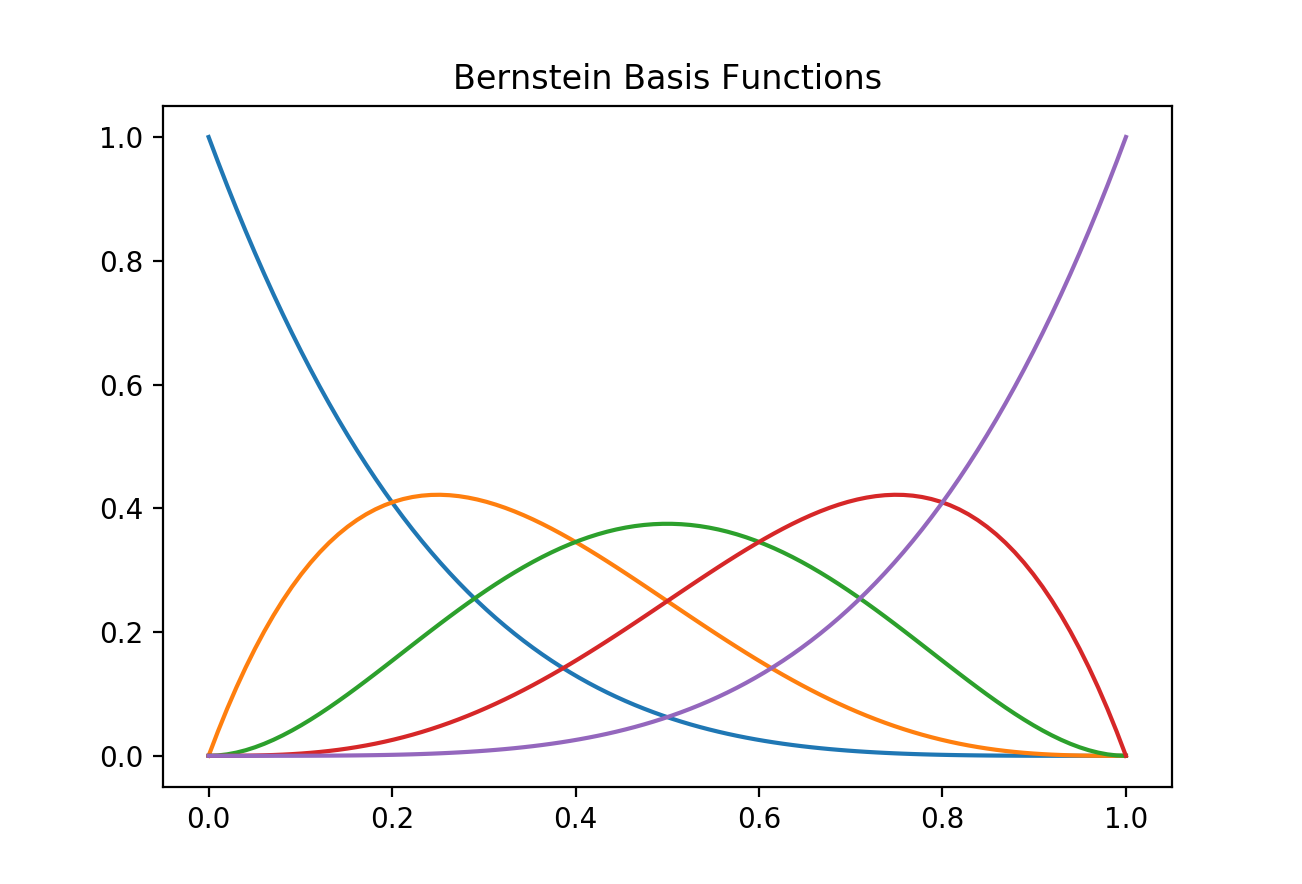
\includegraphics[width=\linewidth]{Basis/basis4}
      \caption{$n=4$}
    \end{subfigure}
    \begin{subfigure}[b]{.45\linewidth}
      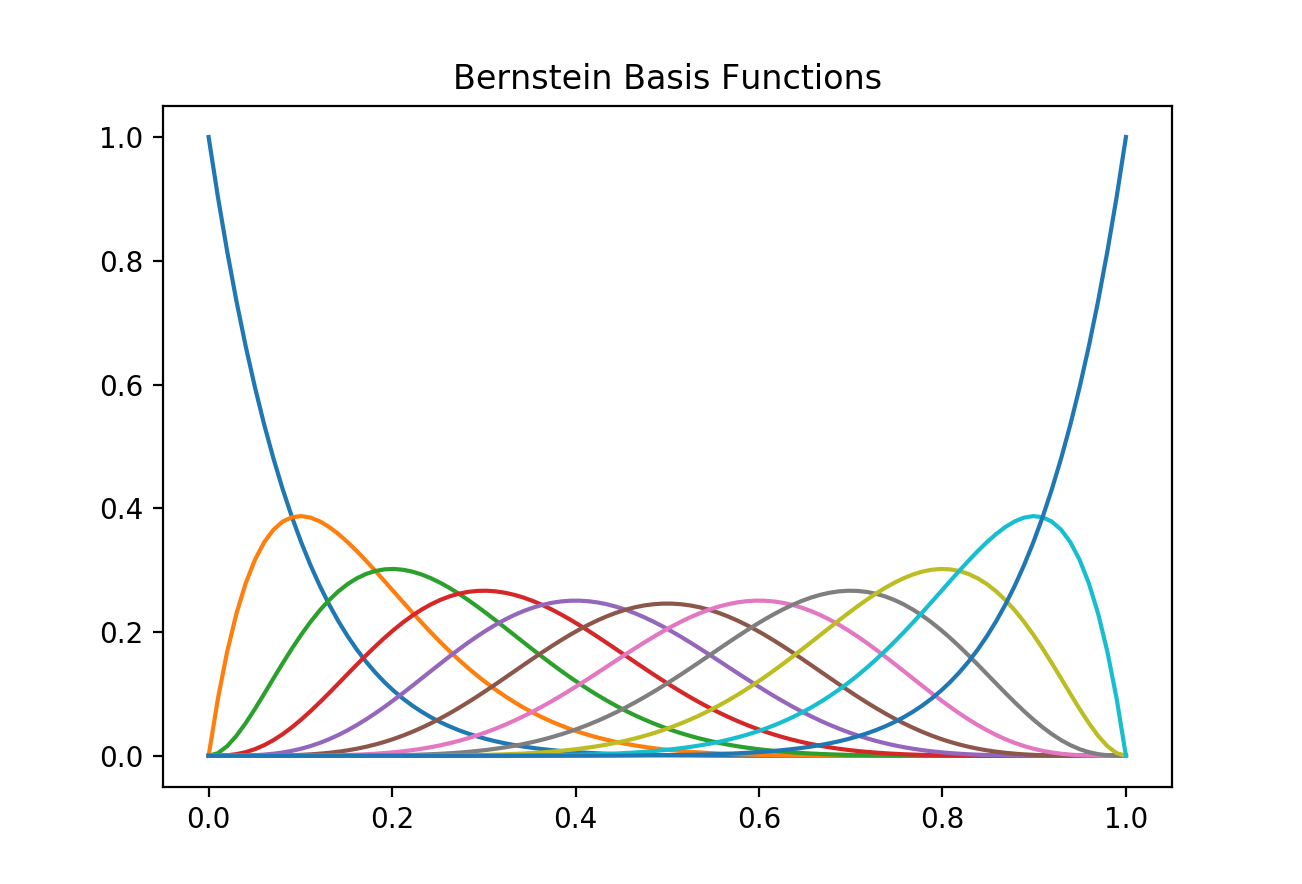
\includegraphics[width=\linewidth]{Basis/basis10}
      \caption{$n=10$}
    \end{subfigure}
  \end{center}
\end{figure}

Bernstein functions are only approximations and to perfectly match the original function you would need an 
infinite degree Bernstein polynomials similar to Taylor series (\ref{eq:BLimit}). The algorithm you use to
generate a B\'ezier curve given your control points is called De Castlejau's algorithm. It is a recursive
algorithm (\ref{eq:DCRec}) that takes your control points and uses them for interpolation. This method is a
little more complicated than the explicit form (\ref{eq:DCExplicit}) which is a summation of the control
points times the basis functions of a given degree $n$. Then to generate any possible curve, parameterize the
X and Y axes and fun De Castlejau's algorithm on the scalar x and y quantities. 

\begin{singlespace}
  \begin{gather}
    \label{eq:DCRec}
    \beta_{n}^{(0)} = \beta_\nu, i = 0,\ldots, n \\
    \beta_{i}^{(j)} = \beta_{\nu}^{(j-1)} (1 - t_0) + \beta_{\nu}^{(j-1)} t_0
  \end{gather}
  \begin{small}
    \begin{itemize}[label=]
      \item $j$ = $1,\ldots,n$
      \item $\nu$ = $0,\ldots,n-j$
    \end{itemize}
  \end{small}
  \begin{equation}
    \label{eq:DCExplicit}
    B(t) = \sum_{\nu=0}^{n} \beta_\nu b_{\nu,n}(t)
  \end{equation}
  \begin{small}
    \begin{itemize}[label=]
      \item $\beta_\nu$: is the $i$th control point
      \item $b_{\nu,n}(t)$: is the Bernstein basis function for the number and degree
    \end{itemize}
  \end{small}
\end{singlespace}

\subsection{Application}
There are a practically infinite number of uses for B\`ezier curves. They and other similar methods are used
to display all curves in computers which means that anything make industrially with a curve has a B\`ezier
curve or other spline involved. However, the hidden ubiquitous use of B\`ezier curves in particular are
fonts. All PostScript fonts, the basis of PDFs, use cubic B\`ezier curves (a) and TrueType fonts,
abbreviated to .ttf, use quadratic curves (b).

\begin{figure}[ht]
  \label{fig:BezierCurves1}
  \caption{Cubic and Quadratic Curves, Listing~\ref{lst:bez}}
  \begin{center}
    \begin{subfigure}[b]{.45\linewidth}
      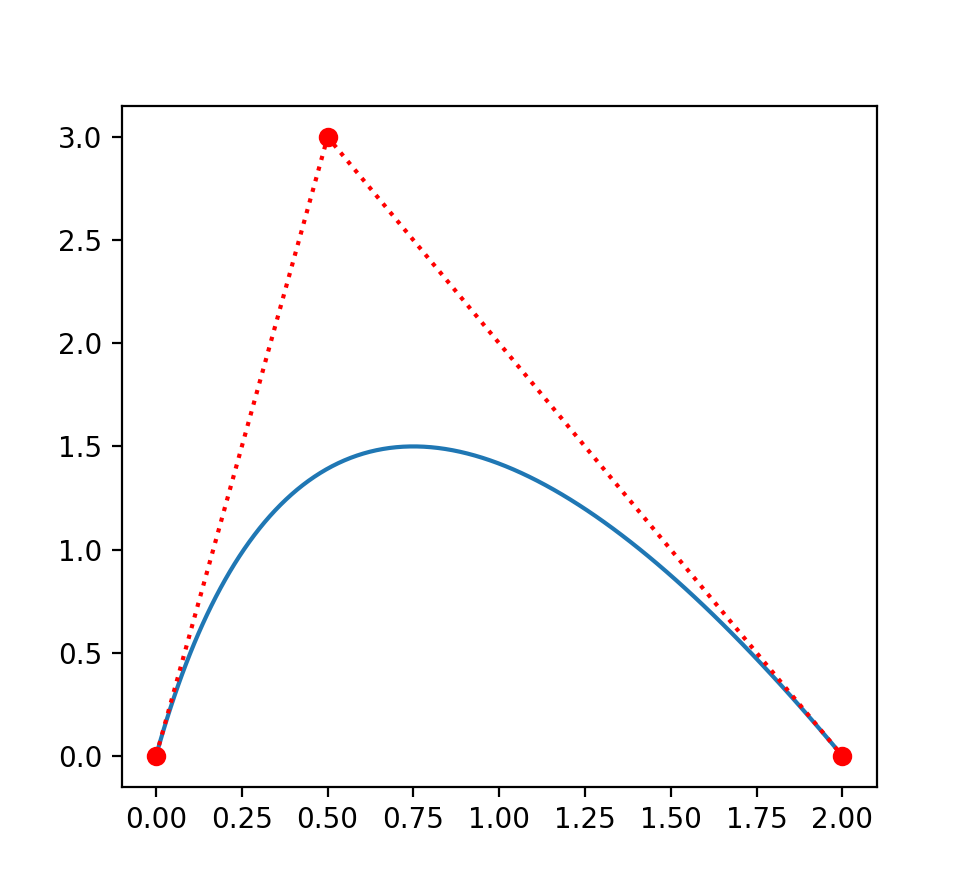
\includegraphics[width=\linewidth]{Bez/cubicBez1}
      \caption{Cubic curve, 3 control points}
    \end{subfigure}
    \begin{subfigure}[b]{.45\linewidth}
      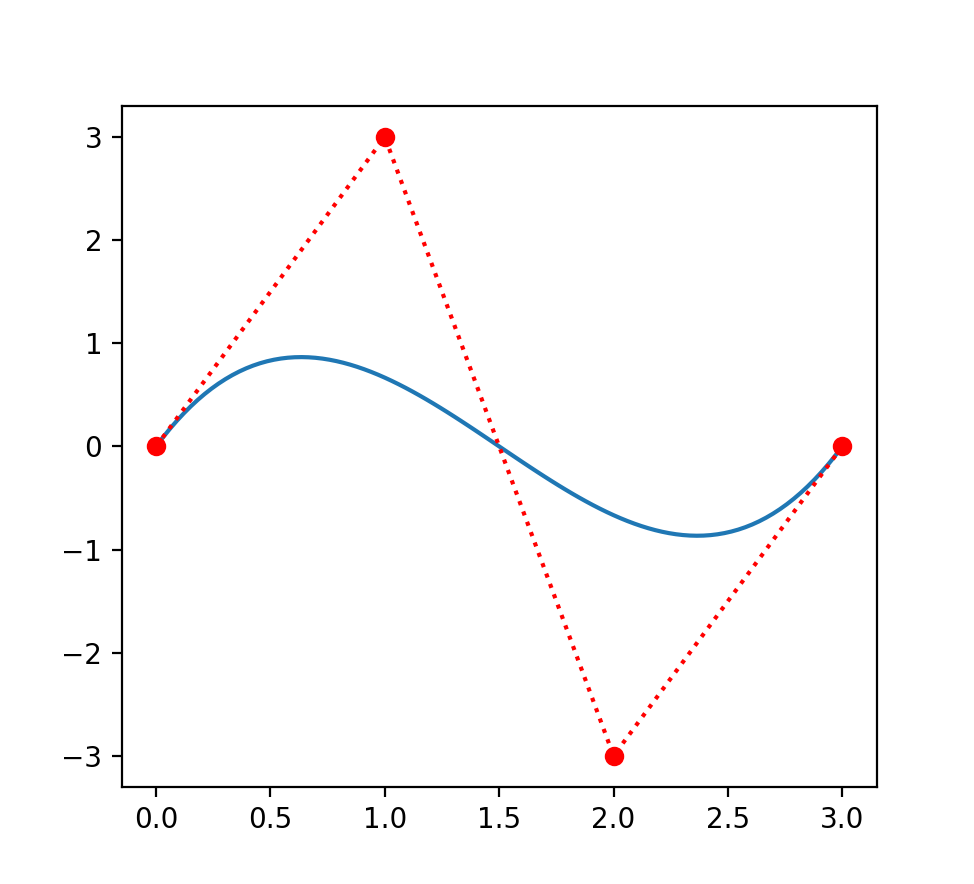
\includegraphics[width=\linewidth]{Bez/quadraticBez1}
      \caption{Quadratic curve, 4 control points}
    \end{subfigure}
  \end{center}
\end{figure}

In fact, most of the computer generated graphics like advertisements contain B\`ezier curves. The popular
software used for such things is Adobe Illustrator\textsuperscript\textregistered which has tools for
generating curves with specific parameters being 2 anchor and 2 control points which is exactly the
quadratic B\`ezier curve. 

The other use for B\`ezier curves are in optimization problems. Since they are used to approximate a 
curve and the control point can be related to the derivative of a function, they are very useful for
optimization problems. They can be used to minimize path lengths \citep{bezierPaths} and can even have
restrictions such as a maximum acceleration or velocity \citep{bezierSoccerPaths}. The acceleration and
velocity limits are caused by the control points which can be controlled since they are tangential to
their anchor points meaning the angle is related to the derivative of the function and the magnitude of
the control point is related to the acceleration or multiple control points. These values can even be 
used to model resistance in a parameterized manner so yet another use of B\`ezier curves would be the
generation of an optimal airfoil \citep{bezierAirfoil}.

\bibliographystyle{apa}
\bibliography{IA}
\newpage
\section{Appendix}
\lstinputlisting[language=Python, label={lst:basis}, caption={Bernstein Basis Functions}]{code/basis.py}
\newpage
\lstinputlisting[language=Python, label={lst:bez}, caption={B\`ezier Curves}]{code/bez.py}

\end{document}
